
\documentclass[letterpaper,10pt]{article}
\usepackage[letterpaper]{geometry} % Importante para que respete el tamaño de papel
\usepackage{array}
\usepackage[english]{babel}
\usepackage[utf8x]{inputenc}
\usepackage{amsmath}
\usepackage{graphicx}
\usepackage{subfig}
\usepackage[colorinlistoftodos]{todonotes}
\usepackage{enumitem}
\usepackage{float}
\usepackage{multicol}
\usepackage{empheq}
\usepackage{csquotes}
\usepackage{physics}
\usepackage{tabularx}
\usepackage{mathtools}
\usepackage{url}
\usepackage{array}
\usepackage{gensymb}
\usepackage{minted}
\usepackage[thinlines]{easytable}
\usepackage{appendix}
\usepackage{wrapfig}
\usepackage{tcolorbox}
\usepackage{etoolbox}
\usepackage{fancyvrb}
\usepackage{listings}
\usepackage{setspace}
\setstretch{1.25}
\usepackage{multirow}
\usepackage{hyperref}


\geometry{
 a4paper,
 total={170mm,257mm},
 left=20mm,
 top=20mm,
 }

\hypersetup{
    colorlinks,
    citecolor=black,
    filecolor=black,
    linkcolor=black,
    urlcolor=black
}

\makeatletter
\newcommand*\@dblLabelI {}
\newcommand*\@dblLabelII {}
\newcommand*\@dblequationAux {}


\usepackage{chngcntr}

\counterwithin*{equation}{section}

\def\@dblequationAux #1,#2,%
    {\def\@dblLabelI{\label{#1}}\def\@dblLabelII{\label{#2}}}

\newcommand*{\doubleequation}[3][]{%
    \par\vskip\abovedisplayskip\noindent
    \if\relax\detokenize{#1}\relax
       \let\@dblLabelI\@empty
       \let\@dblLabelII\@empty
    \else % we assume here that the optional argument
          % has the required shape A,B
       \@dblequationAux #1,%
    \fi
    \makebox[0.5\linewidth-1.5em]{%
     \hspace{\stretch2}%
     \makebox[0pt]{$\displaystyle #2$}%
     \hspace{\stretch1}%
    }%
    \makebox[0.5\linewidth-1.5em]{%
     \hspace{\stretch1}%
     \makebox[0pt]{$\displaystyle #3$}%
     \hspace{\stretch2}%
    }%
    \makebox[3em][r]{(%
  \refstepcounter{equation}\theequation\@dblLabelI, 
  \refstepcounter{equation}\theequation\@dblLabelII)}%
  \par\vskip\belowdisplayskip
}
\makeatother



\newcolumntype{P}[1]{>{\centering\arraybackslash}p{#1}}
\newcommand*\widefbox[1]{\fbox{\hspace{2em}#1\hspace{2em}}}
\newcommand*{\addheight}[2][.5ex]{%
  \raisebox{0pt}[\dimexpr\height+(#1)\relax]{#2}%
}


\newcommand{\multicolinterrupt}[1]{% Stuff to span both rows
\end{multicols}
#1
\begin{multicols}{2}
}

\makeatletter
\AtBeginEnvironment{minted}{\dontdofcolorbox}
\def\dontdofcolorbox{\renewcommand\fcolorbox[4][]{##4}}
\makeatother

\renewcommand{\thesection}{\arabic{section}}
% \renewcommand{\thesubsection}{\thesection.\alph{subsection}}
\renewcommand{\thesubsubsection}{\thesubsection.\roman{subsubsection}}





\special{papersize=8.5in,11in}


\setlength{\parindent}{0pt}

\begin{document}

\begin{titlepage}

\newcommand{\HRule}{\rule{\linewidth}{0.5mm}} % Defines a new command for the horizontal lines, change thickness here

\center % Center everything on the page
 
%----------------------------------------------------------------------------------------
%	HEADING SECTIONS
%----------------------------------------------------------------------------------------

\textsc{\LARGE The University of Sydney}\\[1.5cm] % Name of your university/college
\vspace{2.5cm}
\textsc{\Large ECMT3150 Econometrics of Financial Markets}\\[0.5cm] % Major heading such as course name
\textsc{\large S1C 2022}\\[0.5cm] % Minor heading such as course title

%----------------------------------------------------------------------------------------
%	TITLE SECTION
%----------------------------------------------------------------------------------------

\HRule \\[0.4cm]
{ \LARGE \bfseries Impact of Russian Sanctions on International and Domestic Energy Markets}\\[0.4cm] % Title of your document
\HRule \\[1.5cm]
 
%----------------------------------------------------------------------------------------
%	AUTHOR SECTION
%----------------------------------------------------------------------------------------

%Evan Mak Jhen Wei \hspace{1cm}

\begin{minipage}{0.8\textwidth}
\vspace{0.5cm}
\begin{center}

\textsc{\large Group 1 - The Sanctioneers}\\
\end{center}
\begin{flushleft} \large
\begin{align*}
    \textsc{Aidan Flanagan - 500500516}\\
    \textsc{Alice Deng - 490468734}\\
    \textsc{Baden Spargo - 490431111}\\
    \textsc{Matthew Tonkli - 500506677}\\
    \textsc{Mitchell Rae - 500499601}\\
    \textsc{Utsav Mitra - 490182143}\\
\end{align*}

\vspace{2cm}
\end{flushleft}
\end{minipage}
%~
%\begin{minipage}{0.4\textwidth}
%\begin{flushright} \large
%\emph{Profesor:} \\
%Dr. Ra\'{u}l \textsc{Hern\'{a}ndez} % Supervisor's Name
%\end{flushright}
%\end{minipage}\\[4cm]

% If you don't want a supervisor, uncomment the two lines below and remove the section above
%\Large \emph{Author:}\\
%John \textsc{Smith}\\[3cm] % Your name

%----------------------------------------------------------------------------------------
%	DATE SECTION
%----------------------------------------------------------------------------------------

{\large \today}\\[3cm] % Date, change the \today to a set date if you want to be precise

%----------------------------------------------------------------------------------------
%	LOGO SECTION
%----------------------------------------------------------------------------------------

%\includegraphics{Logo}\\[1cm] % Include a department/university logo - this will require the graphicx package
 
%----------------------------------------------------------------------------------------

\vfill % Fill the rest of the page with whitespace

\end{titlepage} 

\tableofcontents
\clearpage

\section{Introduction}
\subsection{Background}

The present military action in Ukraine began on the 24th of February 2022 following the Russian Federation’s declaration of a “special military operation” in Ukraine \cite{intro1}. In response to this military action, the Russian Federation has been subject to an array of sanctions against individual Russians, Russian businesses, and Russia itself. Many of these sanctions directly target Russian oil and natural gas production, as well as the ability of Russia to sell this oil and natural gas to neighbours.
\medskip

Russia is a major entity in the global energy market. Russia is the third largest oil producer, accounting for ~12\% of global oil production, and is the second largest gas producer, accounting for ~17\% of natural gas production globally \cite{intro2}, thus, the impact of sanctions aimed at limiting the scale at which Russia is able to produce and export oil and gas is likely to have had a significant impact on the markets for these key commodities. Since the beginning of the war, the United States and Canada have banned Russian oil imports, whilst many other nations have specifically targeted sanctions and oil and gas producing companies in Russia. This is expected to both affect the global prices of oil and gas as well as the volatility of these prices, due to the rapidly changing nature of these sanctions.

\subsection{Aim}

This report will examine the impact of oil and gas related sanctions imposed upon the Russian Federation on the volatility of the price for crude oil and liquid natural gas (LNG) in both global and domestic (Australian) markets. We examine these impacts through the creation of a GARCH(1, 1) model, which was specified according to both relevant econometric literature and statistical tests. We then fit this model to the global prices of crude oil and liquid natural gas, and compare the realised level of volatility in these markets to a counterfactual generated by the specified model in the absence of sanctions, quantifying the expected magnitude of volatility in this forecast to the realised volatility in these markets, with sanctions in place. Additionally, we examine the possible impacts that sanctions on Russian gas exports may have on the price of electricity in Australia using a multivariate vector autoregressive model, and explore the possibility of a cointegrating relationship between global oil and gas spot prices to examine the possible impacts that sanctions on one commodity may have upon the other.
\medskip

Such an analysis is of interest to econometricians and policy makers alike as we aim to quantify the effect of a coordinated campaign of sanctions and economic warfare against a large oil and gas producing nation on the prices of oil and gas – critical commodities that impact the costs of producing and transporting a significant quantity of global goods and services, impacting all sectors of the global economy. In the Australian context, such a report is of interest as we examine the magnitude to which the Australian oil and gas markets are sensitive to sharp exogenous changes in the global prices of oil and gas.

\section{Literature Review}
The sanctions imposed on Russia in response to its invasion of Ukraine have had an impact on gas and oil markets due to Russia’s position as a major producer of both commodities. Quantitative data is commonly used to forecast and explain changes in these oil and gas markets, including in response to shocks from sanctions on producing countries. In this review, the possible outcomes and ongoing effects of the current sanctions imposed on Russia will be explored through an analysis of previous papers that investigate the workings of these markets in response to sanctions and other shocks. These papers will be used to assess the relationship between sanctions and other shocks on the price and volatility of oil and gas. The findings from the studied papers will provide a helpful context and background understanding to the statistical modeling to be undertaken to assess the unique impact which the recent Russian sanctions are having upon these markets.
\medskip

Brown \cite{aid1} analysed the effects of the United States’ sanctions imposed on Iran, Russia, and Venezuela, as of 2020, and found them all to have some effect on oil markets. Brown found the effect that the sanctions had on global oil markets was dependent on the target and thoroughness of the sanctions. Another important factor was the design elements in the sanctions specifically designed to avoid global impacts by certifying that oil markets outside of the sanctioned country were adequately supplied. In the examples discussed in this paper, these included coordinating with oil-producing nations, significant reduction exceptions for industries defined as critical, and ‘wind-down’ periods after the imposition of the sanctions. While these approaches attempted to reduce the global impact on oil markets, in the case of the Iranian and Venezuelan sanctions, which did cause an immediate drop in oil production, the global price of oil did rise. However, likely due to these design elements, as Brown hypothesises, the price soon adjusted as other oil-producing nations increased production. While this paper does analyse the effects of sanctions on global oil markets, there is little empirical data analysing this effect, thus it is hard to understand to what amount these sanctions had an effect, or to apply the data to any past or future sanction events. In the case of the recent sanctions on Russia, which have affected Russian oil production and its ability to export more than the sanctions which started in 2014, this paper gives little insight into the effect of these sanctions, considering the greater amount of global oil production which is being impacted by them. Due to the rapid nature of Russia’s recent sanctions, this article would imply a larger effect, as there was not enough time to ensure adequate supply and design the sanctions so as not to have such a large effect. While this article offers little insight into the empirical relationship between oil markets and sanctions, it does establish a strong relationship between them, informing the research in this paper.
\medskip

In their article, Mohaddes and Pesaran \cite{aid2} try to quantitatively assess the impact of country-specific oil shocks on the global economy using a counterfactual analysis. They have used various vector autoregressive (VAR) models to find the relationships between price shocks in one country and the global oil price. By specifying the model to a Global-VAR model, the findings are able to specifically analyse the effects of a country-specific shock, thus considering the actions of other oil-producing nations in response. This paper is then able to deliver specific empirical insights into the effects of a country’s shock, such as the recent Russian sanctions, on the global oil market. They find that when the affected country produces large amounts of oil, there is far less spare capacity in other producing nations, and the oil markets can be affected. The example of Saudi Arabia is used, the largest oil-producing nation at the time of writing (and still a very significant one \cite{aid3}). Using their model, with an 11\% long-run reduction in oil production, it results in a price increase of 22\% in oil. Russia’s production from February (pre-invasion) to March appears to have dropped by a fiftieth of that \cite{aid4}, but utilising the approach of this paper, the impact of Russia’s sanctions can be isolated within its effect on the global markets. Other approaches to control for confounding variables include the synthetic control method, discussed by Abadie, Diamond, and Hainmueller \cite{aid5}, in which an aggregate of other indicators are used to simulate the affected country.
\medskip

Both of these papers provide justification for the research question this report poses, and suggest there should be some effect on global oil and gas prices due to the imposition of sanctions that target their ability to produce and export these commodities. The econometric analysis in Mohaddes and Peseran’s paper provides evidence of a VAR model being appropriate when conducting a counterfactual analysis, however, as discussed in their paper, the VAR model has limitations. It cannot account for as many time series data as a GARCH model and is not able to accurately model data for both oil and gas data which is the goal this report. The GARCH(1,1) used to conduct the analysis in this report is based upon this research as well as other findings and patterns identified through data inspection into the prices of these commodities.

\section{Data Description}

We have selected the daily spot price of Brent crude oil and the daily Gas Supply Hub (GSH) \cite{mitch1} trade price of LNG as measures of the price of oil and natural gas in Australia. Brent crude in this context refers to both the dated price of a basket of North Sea crude oils and the contract price of Brent crude oil futures \cite{mitch2}. Whilst the price of South-East Asian crudes such as Malaysian Tapis became a benchmark for Asia-Pacific oil markets in the 1990s, decreasing regional production in past decade have resulted in the establishment of Brent crude as Australia’s benchmark price \cite{mitch3}. 
\medskip

GSH trade price refers to an average of wholesale LNG trade prices across the two AEMO operated gas supply hubs in Wallumbilla, Queensland and Moomba, South Australia \cite{mitch1}. These wholesale trade prices largely function as a benchmark for LNG price across east coast Australia and capture factors such as domestic demand and netback price, the equivalent export value price of LNG \cite{mitch4}.
\medskip

As this report is primarily interested with sanction-driven price patterns, the 21 February 2022, the introduction of sanctions specifically in response to what has become the invasion of Ukraine, has been selected as the point of divergence. Daily data for the two years up to 21 February has been selected to construct the model. Furthermore, 2022 data is available up to 16 May in the case of both oil and LNG. The Brent crude oil dataset is fairly clean yet still contains some missing values. Due to the daily frequency and number of years available it is judged that there is sufficient data to drop these missing values. The monthly LNG hub price dataset is comparatively messy with isolated price spikes and additional price forecasts. These isolated spikes are an undesirable result of using monthly data, however, a lack of transparency within the Australian gas market, results in difficulty finding higher frequency data. To counteract this, it was decided more years of LNG data were to be included in the modelling to compensate. The dataset is otherwise complete, and the forecast data can be dropped.

% Brent Crud price over time

\begin{figure}[H]
    \centering
    \subfloat[\centering Brent Crude price]{{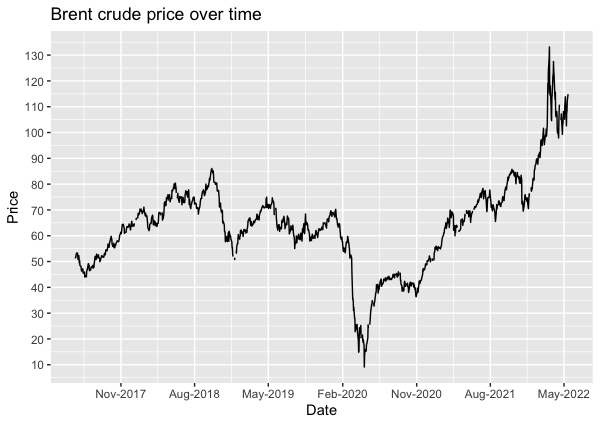
\includegraphics[width=7cm]{Figures/Data-desc/Brent-crude-price.png} }}%
    \caption{Brent Crude price between late 2017 and mid 2022}%
    \label{fig:Brent-Crude-price}%
\end{figure}

\subsection{Time Series Visualisation}

Visual analysis of our Brent crude data reveals a steady two year trend before a clear period of increased price volatility beginning on 25 February 2022. This is most evident over March there are two large price spikes and subsequent drops. The largest of these saw price increasing from \$103.08 USD per barrel to over \$133 USD in eight days. This spike coincides with the exclusion of select Russian banks from the SWIFT system on the 26th \cite{mitch5}, and the sale of BP’s 19.75\% stake in state-controlled oil company Rosneft on the 27th \cite{mitch6}. Notably, there is a four day delay between the initial introduction of tariffs and this price jump, suggesting the Russian invasion on the 24th as a more likely cause. The presence of these spikes late in our dataset also suggest heteroskedasticity as a potential issue. By selecting 21 February as the cutoff date for our counterfactual forecast data we do not include this late period of volatility, thus avoiding this late onset heteroskedasticity.

\begin{figure}[H]
    \centering
    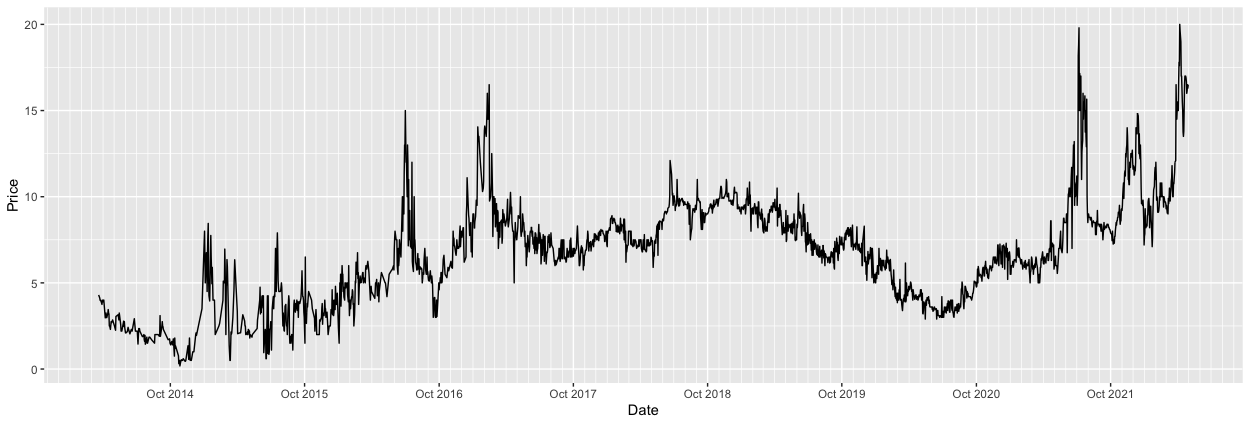
\includegraphics[width=.8\textwidth]{Figures/Data-desc/GSH trade price.png}
    \caption{Results bar graph}
    \label{fig:GSH-trade-price}
\end{figure}

By comparison, our LNG dataset does not appear to show a clear pattern of post invasion pricing. Historical GSH data shows a price fall from around \$12/GJ in late February 2022 to \$9/GJ in early March, followed by a spike of \$10/GJ until early April. Despite this, there is evidence of similar price rises and falls occurring even before the introduction of sanctions and the invasion of Ukraine. From October to December 2021 wholesale Australian prices approximately doubled, largely in response to upward demand for LNG from Asia in expectation of a colder Northern Hemisphere Winter \cite{mitch7}. The instance of sudden December price rises occurring in 2014, 2016 and 2021 could indicate some seasonality but the lack of a consistent yearly pattern is counter-intuitive. Visual analysis of seasonality in our LNG price data is thus inconclusive. As before, volatility increases throughout 2022, the end of our dataset, suggesting that heteroskedasticity remains a concern. This is also partially avoided by removing post-sanction data when constructing our forecast.

\subsection{Augmented Dickey Fuller Test}

\begin{table}[H]
\centering
% \setlength{\tabcolsep}{5pt} % Default value: 6pt
% \renewcommand{\arraystretch}{1.5} % Default value: 1
\caption{Augmented Dickey-Fuller Test Results}
\begin{tabular}{c|cc}
            & No Trend & Trend\\\hline\hline
Brent Crude & -1.7373 & -2.5021\\\hline
Henry Hub & -2.5264 & -4.3439**
\end{tabular}\label{Tab:ADF_LNG}
\\
* Significant at the 5\% level\\
** Significant at the 1\% level
\end{table}

We test both datasets for autocorrelation using an augmented Dickey-Fuller (ADF) test with and without trend. Akaike information criteria suggests selecting lags equal to one. Results from the ADF test suggests there is only statistically significant evidence of trend stationarity in our LNG supply hub price data.

\subsection{ADF and PACF Visual Analysis}

\begin{figure}[H]
    \centering
    \subfloat[\centering LNG netback ACF]{{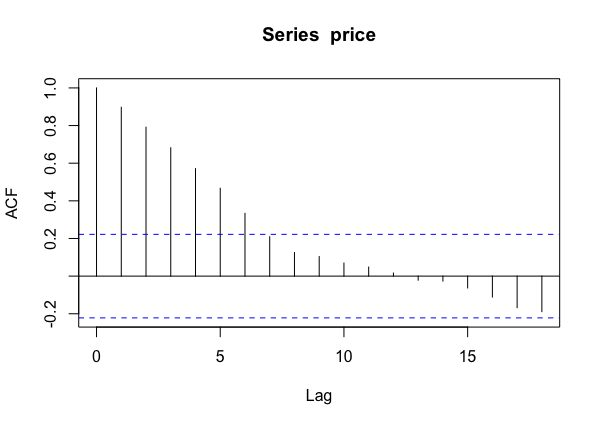
\includegraphics[width=0.4\textwidth]{Figures/Data-desc/LNG netback ACF.png} }}%
    \qquad
    \subfloat[\centering LNG netback PACF]{{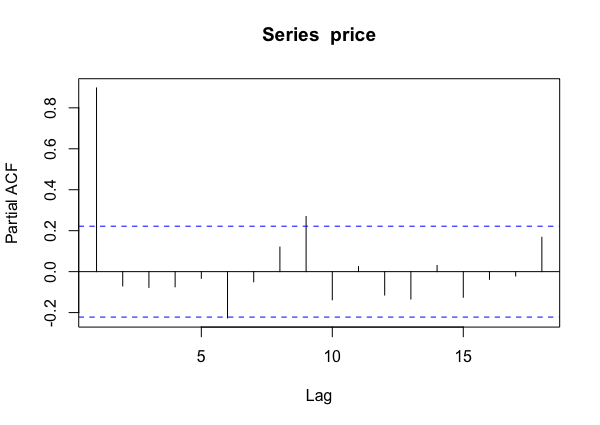
\includegraphics[width=0.4\textwidth]{Figures/Data-desc/LNG netback PACF.png} }}%
    \caption{LNG netback}%
    \label{fig:example3}%
\end{figure}

Analysing our ACF for our Brent crude data reveals a decay to zero, suggesting at least some minimal stationarity despite not finding statistically significant evidence in our ADF test. Furthermore, whilst there are comparatively large lags in our PACF there appears to be no clear seasonal pattern. This would support the conclusion there is little seasonality in crude oil prices.

\begin{figure}[H]
    \centering
    \subfloat[\centering GSH trade price ACF]{{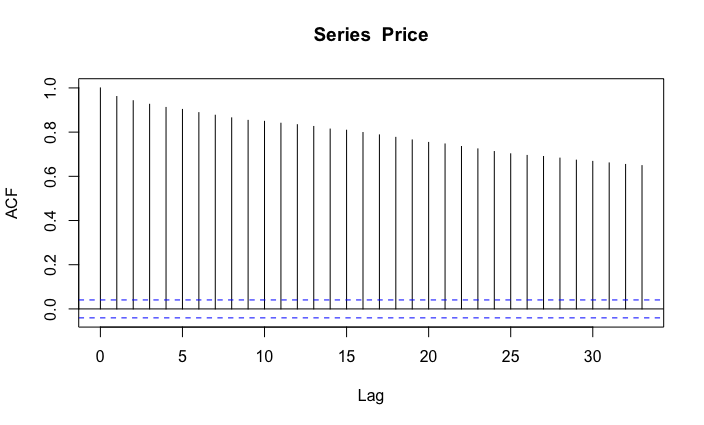
\includegraphics[width=0.4\textwidth]{Figures/Data-desc/GSH trade price ACF.png} }}%
    \qquad
    \subfloat[\centering GSH trade price PACF]{{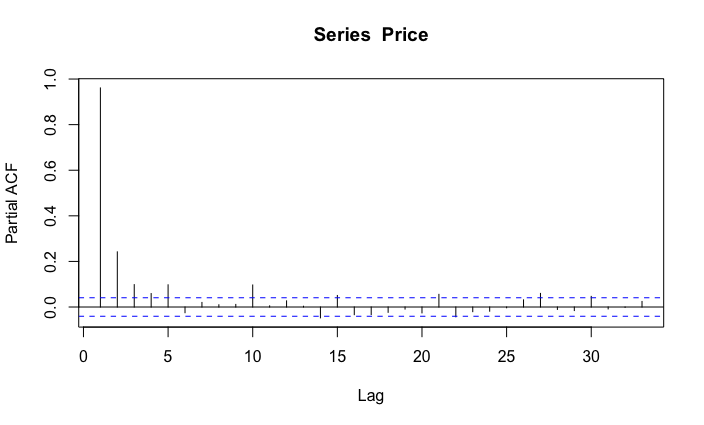
\includegraphics[width=0.4\textwidth]{Figures/Data-desc/GSH trade price PACF.png}{F} }}%
    \caption{GSH trade price}%
    \label{fig:example4}%
\end{figure}

Our LNG supply hub price data shows an even more gradual linear decay in the ACF as would be expected from non-stationary data. This is consistent with the trend-stationarity identified in our ADF test. The PACF graph illustrates a muddied pattern of larger lags decaying occurring at 5, 10, 15, 21, and 27 after an initial decay from 1. This averages out to a season of about 5-6 months. This is reasonable considering the 6 month delay between Southern and Northern hemisphere winters, which could explain these seasonally higher gas prices. Despite this, given a lack of corroborating evidence in our ACF and time series graph suggests this seasonality is likely spurious.
\medskip

Overall, we find both our Brent crude oil and our supply hub LNG trade price data is largely non-stationary. Despite this, ADF test results suggest LNG price may be stationary when de-trended. We find insufficient evidence of seasonality in either dataset.
\section{Analysis of Gas in the Australian National Electricity Market}

In this section we will be taking a closer look at the significance of Gas in Australia’s Domestic National Electricity Market (NEM). The NEM is one of the biggest distributed energy systems in the world and is the deregulated portion of Australian energy, and hinges on an efficient market. We will conduct our study on Gas consumption price to national average spot energy price and compared to other means of electricity generation, this will be done using Multivariable Vector Autogregression model (MVAR) and using quantity consumed and average spot prices.

\subsection{Observations}

Energy consumption data in NEM is gathered from AEMO \cite{NEM1} combined with OpenNEM \cite{NEM2} is categorized by the top 11 energies consumed:

\begin{multicols}{4}
\begin{itemize}
    \item Battery (Discharging)
    \item Wind
    \item Solar (Utility)
    \item Solar (Rooftop)
    \item Hydro
    \item Coal (Brown)
    \item Coal (Black)
    \item Gas (Steam)
    \item Gas (CCGT)
    \item Gas (OCGT)
    \item Gas (Reciprocating)
\end{itemize}
\end{multicols}

\begin{figure}[H]
    \centering
    \subfloat[\centering Stacked Barplot of GigaWatt hours energy consumed ]{{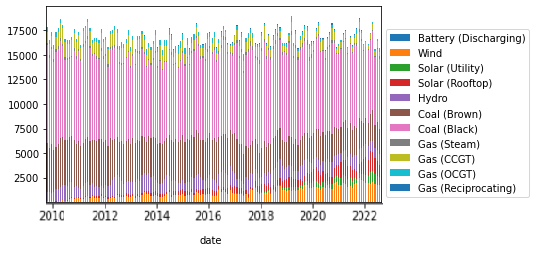
\includegraphics[width=0.4\textwidth]{Figures/NEM-Analysis/consumption.png} }}%
    \qquad
    \subfloat[\centering Price of each energy per GigaWatt ]{{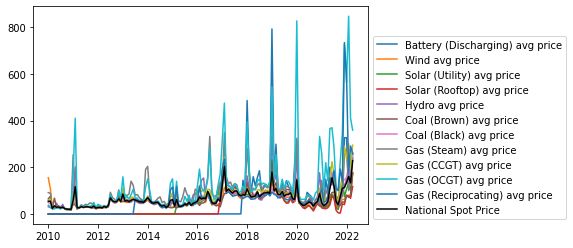
\includegraphics[width=0.4\textwidth]{Figures/NEM-Analysis/price_gigawatt.png} }}%
    \caption{figures for every month 2009-2022}%
    \label{fig:NEM-consump-price}%
\end{figure}

As a general overview, we can see there is cyclical pattern of aggregate consumption where the barplot display a cyclical pattern, this is different to global analyses and could be because of physical weather and seasons. Another observation is the use of Hydrocarbons (such as gas and coal) generally decreasing over time, which is opposite to renewable energies, particularly wind and solar, which are growing over time.
\medskip

Some particular observations are that different states have varying reliance on gas, for example Tasmania, which has so much excess supply of hydro electricity that it will export it to the NEM where it can be sold. Another observation is how South Australia's reliance on gas has decreased over time: in October 2009 it accounted for 61\% of the state's consumption but recently as of April 2022 it accounts for 20\%, compared to its renewable energy (combined Solar and Wind) consumption which accounts for 62\%.

\subsection{Data Preparation}

Though it is interesting to see specific observations like in our previous section, we will be using average spot prices as we are looking for significant systematic effects rather than special local cases.
\medskip

Since in figure \ref{fig:NEM-consump-price}.b, we observe that some Gas prices are 0 until 2018, we will focus from 2018 until present. We will also aggregate the different types of gas and combine their market value and energy consumption to model the aggregate effect of gas compared to the other energies. 
\medskip

To compare the impact of each energy source in the market we first need to convert each energy to its average spot price which we do by dividing aggregate market value and aggregate market consumption in terms of Australian Dollar per MegaWatt hours: 

\begin{equation*}
    \text{Average Energy Spot Price}=\frac{\text{Aggregate Energy Market Value}}{\text{Aggregate Energy Market Consumption}}
\end{equation*}
\medskip

After this is done, the energies prices are now comparable to each other. For the Vector Autoregression model to be fitted well, we need to enforce weak stationarity. For each energy timeseries, we attempted to enforce weak stationarity by normalizing subtracting its mean and divided by its standard deviation, and noticed yearly variance thus divided every year by its yearly variance to remove unfavourable seasonal volatility.

\begin{figure}[H]
    \centering
    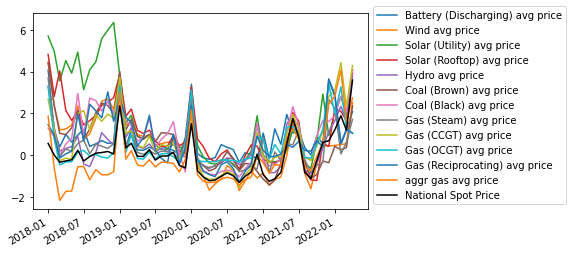
\includegraphics[width=0.6\textwidth]{Figures/NEM-Analysis/prep_data.png}
    \caption{Prepared Average spot price for each energy every month 2018-2022}
    \label{fig:NEM-avg-price}
\end{figure}

\subsection{Multivariate Vector Autoregression and Discussion}

Firstly, we run a Partial autocorrelation on national spot energy price to decide how many lags we should focus on. We find an AR(13) model with strong seasonality especially with 12th lag, this makes sense as last year's physical weather and season would be the most similar and thus, most significant.

\begin{figure}[H]
    \centering
    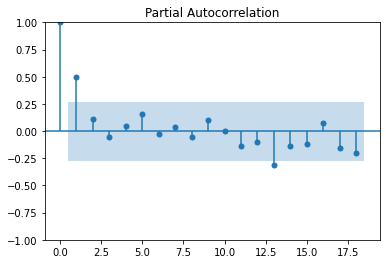
\includegraphics[width=0.6\textwidth]{Figures/NEM-Analysis/PACF-national.png}
    \caption{PACF of National Energy Spot Price}
    \label{fig:NEM-avg-price}
\end{figure}

Since we know NEM spot pricing is composed of the energies of interest, they are endogenous, and can be used to be modelled by a Multivariable Vector Autogregression model (MVAR). The function we run optimizes over AIC and BIC information criterion and gives us the following correlation matrix of residuals:

\begin{figure}[H]
    \centering
    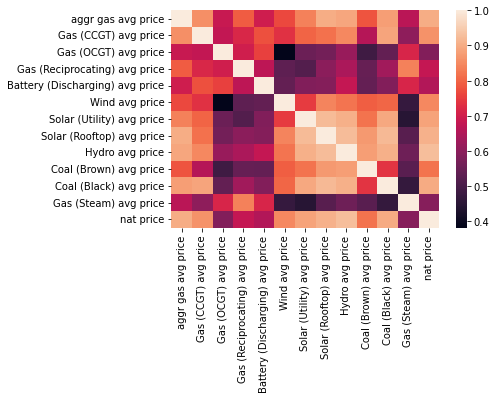
\includegraphics[width=0.6\textwidth]{Figures/NEM-Analysis/correl_var.png}
    \caption{Correlation Matrix of Residuals}
    \label{fig:NEM-correl}
\end{figure}

Observing results gives us a big MVAR model, which is overparameterized and not very useful for further prediction. However, we can compare relative effectiveness of each energy to each other. The correlation residuals show that national spot energy price has the highest correlation with Hydro and Solar Rooftop energy, but Lowest correlation with Gas STEAM and Gas OCGT. However, the spot price has a moderately high correlation to Aggregate gas pricing. This could be because gas STEAM is highly efficient but hard to provide consumption on demand, which is opposite to Gas OCGT where it is less efficient, but generators can be turned on almost instantly. Since these are aggregated, they provide a hedge to each other thus following the national spot price more closely.
\medskip

In this ad hoc MVAR analysis we find that individual gas price is not a great predictor of national spot price and aggregate gas spot price is only moderately correlated. Thus, international gas price fluctuations will have very minimal direct effect on domestic electricity generation from gas. Further analysis and more intensive modelling, perhaps incorporation of weather and seasonal data is required for more conclusive results.
\section{GARCH}
\subsection{Model Justification}
Volatility in financial markets is a key indicator for assessing risk and is crucial in forecasting future values. The sanctions imposed on Russia following its invasion of Ukraine on 24 February 2022 heavily impacted the European energy market as Russia was the main supplier of natural gas in the region. Extreme volatility in the energy market has been observed since, as the market responds to these ongoing sanctions. When looking closely at the Australian energy market to assess the responses of the domestic natural gas and crude oil markets to Russian sanctions, historic volatility modelling is useful in helping us predict how the markets would have performed sans sanctions.
\medskip

The LNG and oil markets are inherently volatile commodities as they are primarily driven by market-specific demand and supply shocks as well as structural shocks. The nature of the markets means that we cannot assume a state of constant volatility as the prices fluctuate based on specific forces. Extensive literature review has shown that on forecasting commodities such as natural gas and crude oil, recent studies have commonly used models that allow for regime switching after a certain threshold such as Self-Exciting Threshold AutoRegressive (SETAR) and variations of Generalised Autoregressive Conditional Heteroskedasticity (GARCH) models \cite{alice1}. For example, Ngyuen and Nabney \cite{alice2} used GARCH models combined with linear regressions and Artificial Neural Networks (ANN) to forecast natural gas prices; Lv and Shan \cite{alice3} used non-linear GARCH type models as part of their analysis and research into the volatility of natural gas prices. There is a clear precedence of the usage of econometric models, in particular GARCH model variations, in analysing the volatility of commodities such as natural gas and crude oil in practice, which sets the stage for the model selected in this project.
\medskip

The GARCH model is designed to help produce a measure for volatility. These autoregressive processes depend on past observations and variances in modelling for current and future variances. A feature of the GARCH model that makes it relevant to use in forecasting energy markets such as LNG and crude oil is that these models do not assume constant volatility. For a more realistic model, GARCH models are designed in a Bayesian framework with a learning behaviour in place to use the most recent standard deviation of returns. By aiming to minimise prediction errors by accounting for errors in prior forecasting, the accuracy of the predictions is more enhanced, which is why a GARCH model was selected for forecasting LNG and crude oil prices.

\subsection{GARCH Model: GSH Market}

The dataset contains 8 columns of data, however only 2 are needed: the trade data and the price of the trade. Once we have filtered these columns, we need to create a new column for the percent change for the day-to-day prices. These measures were done using the Pandas library in Python. 
\medskip

The returns on the prices were then squared under an additional column for running the GARCH model fit on.
\begin{figure}[H]
    \centering
    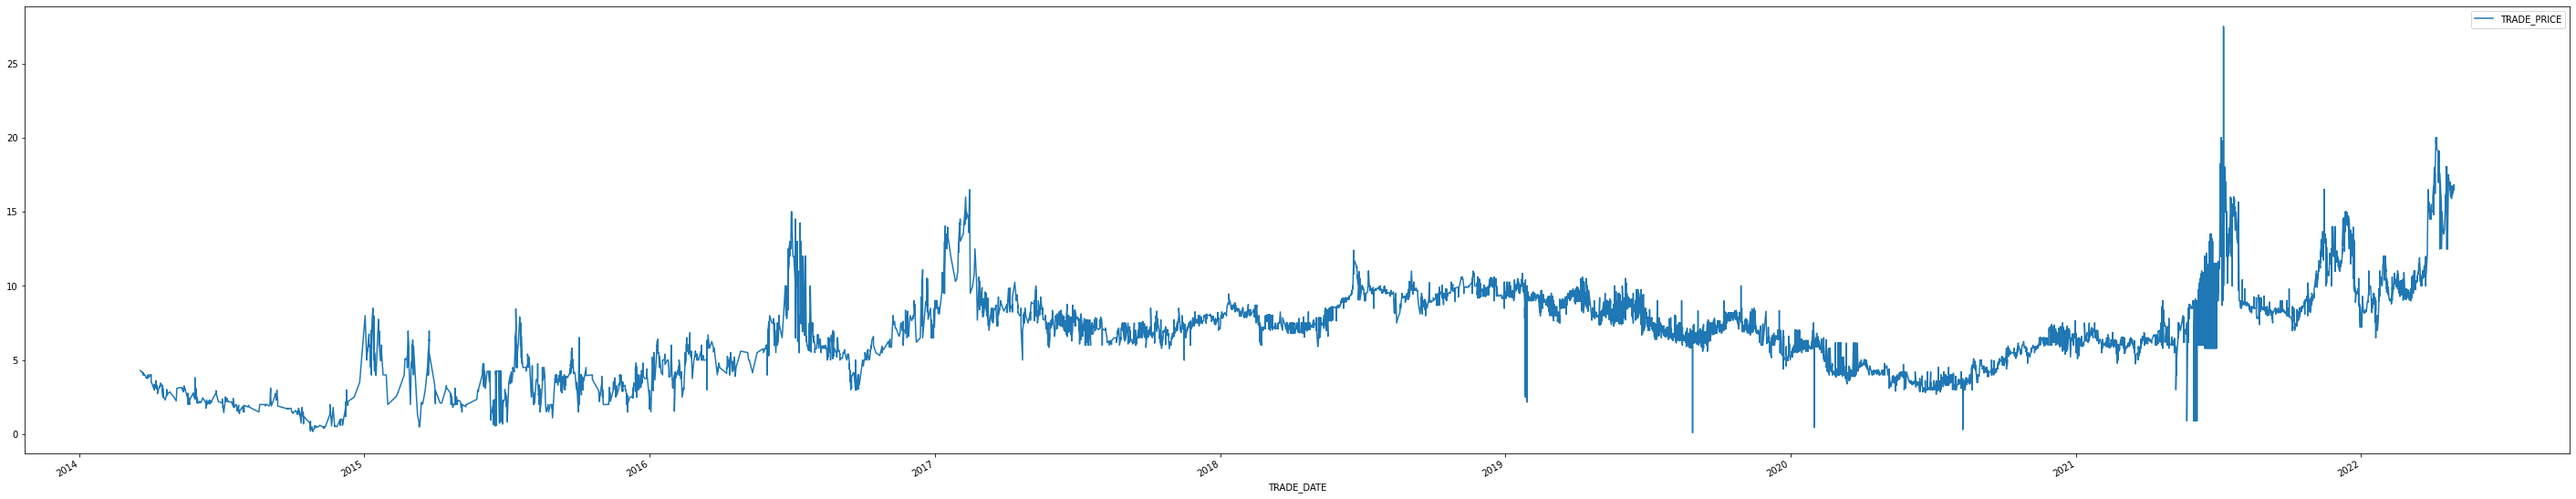
\includegraphics[width=1.0\textwidth]{Figures/Garch/gas.png}
    \caption{Daily GSH Returns Plot}
    \label{fig:Results_table}
\end{figure}

We found a GARCH(1, 1) model to fit the best, obtaining statistically significant p-values and t-test scores, as well as a relatively low AIC and BIC when compared to other GARCH mode parameters.
\begin{figure}[H]
    \centering
    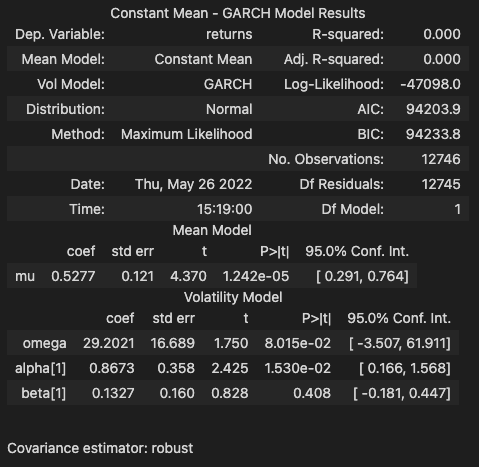
\includegraphics[width=0.5\textwidth]{Figures/Garch/garch.png}
    \caption{GARCH(1, 1) for GSH Market}
    \label{fig:Results_table}
\end{figure}

\subsection{GARCH Model: Brent Crude Oil}
\begin{figure}[H]
    \centering
    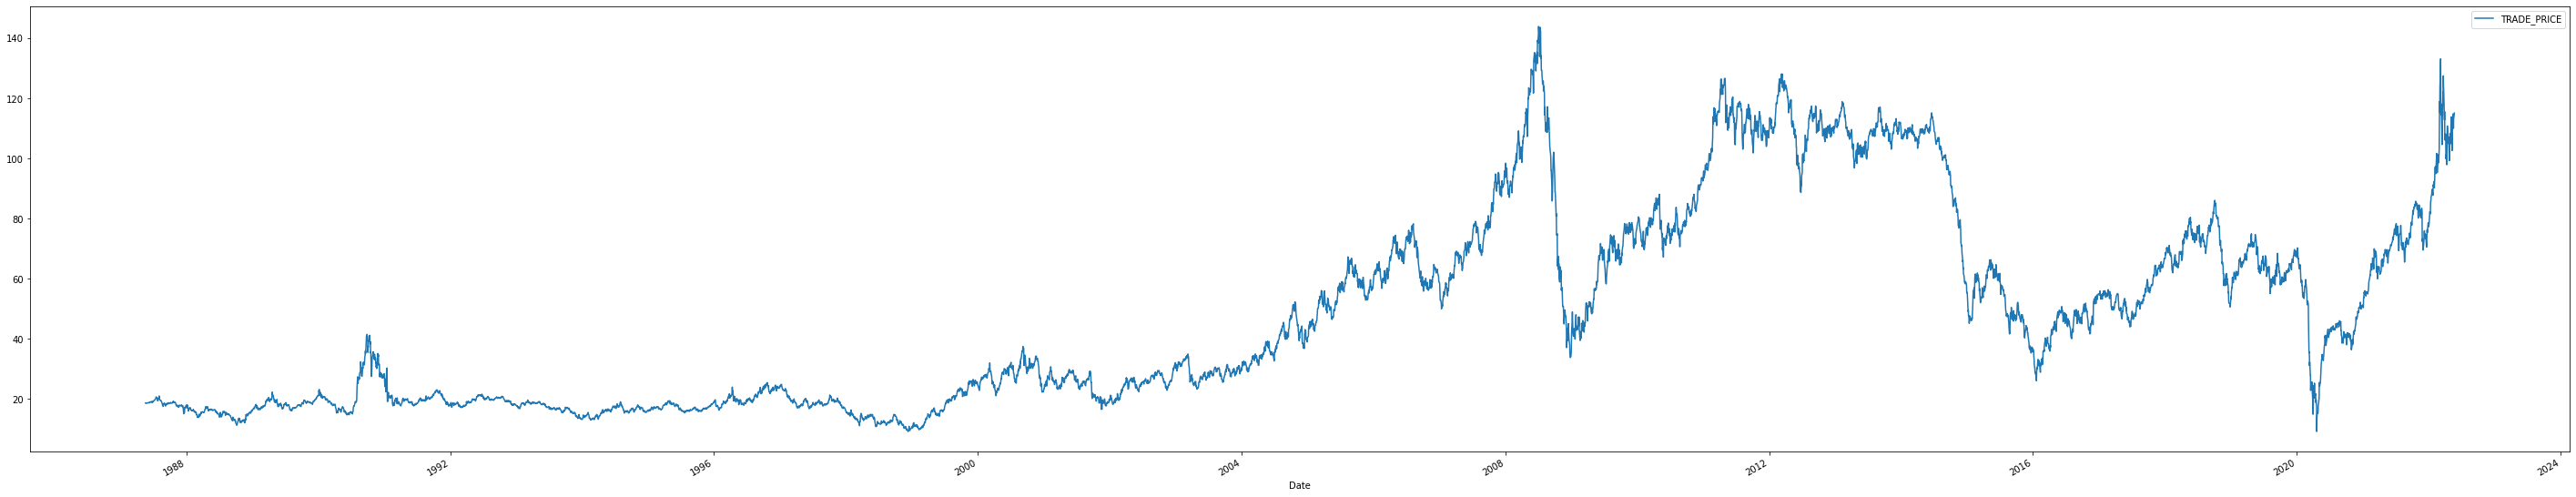
\includegraphics[width=1.0\textwidth]{Figures/Garch/brent.png}
    \caption{Daily Brent Crude Oil Returns (Dollar per Barrel) Plot}
    \label{fig:Results_table}
\end{figure}
The data for crude oil was of a daily frequency and did not need much wrangling or modification for the model. However, we created a column for daily percent returns for the price on dollars per barrel of crude oil. Following the same process as the GSH data, we were able to attain a GARCH(1, 1) model with competent p-value and t-test values as well as a low AIC and BIC. 
\medskip

\begin{figure}[H]
    \centering
    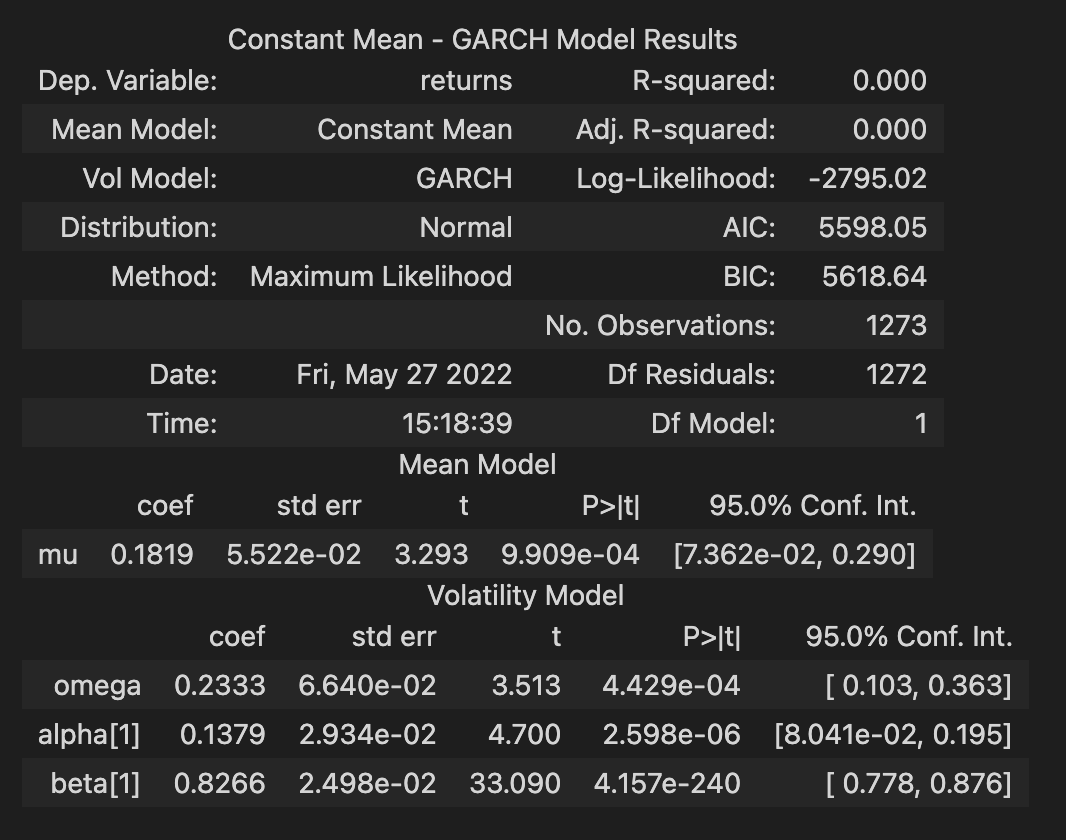
\includegraphics[width=0.5\textwidth]{Figures/Garch/crude.png}
    \caption{GARCH(1, 1) Model for Brent Crude Oil Market}
    \label{fig:Results_table}
\end{figure}

\subsection{Annualised Conditional Volatility}
The following are the standardised residuals and the annualised conditional volatility for the GSH Market and the Brent Crude Oil Market:
\begin{figure}[H]
\centering
\begin{minipage}{.5\textwidth}
  \centering
  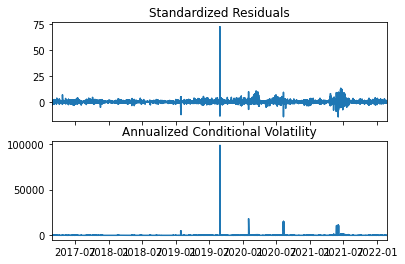
\includegraphics[width=1.0\linewidth]{Figures/Garch/gas_annualised.png}
  \label{fig:test1}
\end{minipage}%
\begin{minipage}{.5\textwidth}
  \centering
  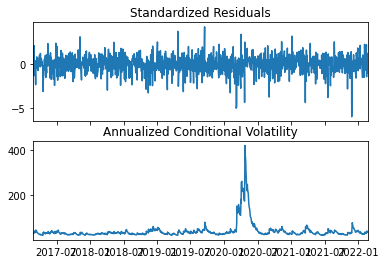
\includegraphics[width=1.0\linewidth]{Figures/Garch/crude_annualised.png}
  \label{fig:test2}
\end{minipage}
\end{figure}

\subsection{Forecasting Volatility}
We then mapped the volatility and forecasted it for the remainder of each of the datasets past the date of the Russian sanctions being imposed. For the Gas Supply Hub this was 68 days of forecasting and 91 days for the Brent Crude Oil. We mapped this forecast along with the volatility of the realised values of both datasets.
\begin{figure}[H]
    \centering
    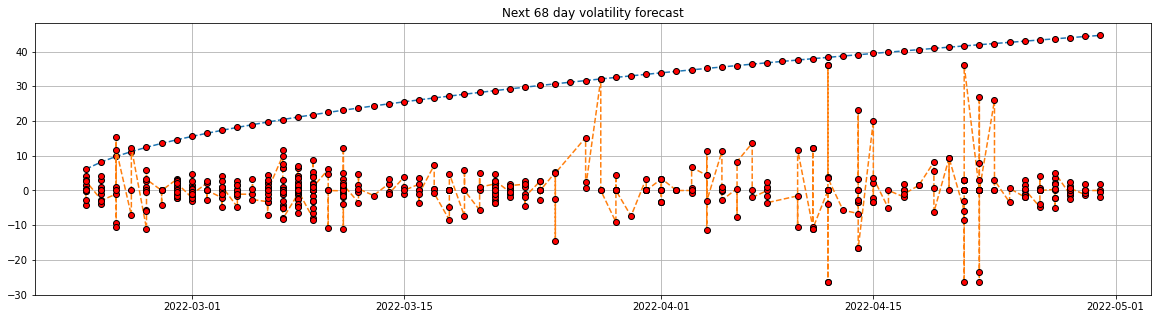
\includegraphics[width=0.6\textwidth]{Figures/Garch/gas_forecast.png}
    \caption{GSH Market Volatility Forecast with Realised Values}
    \label{fig:Results_table}
\end{figure}
\begin{figure}[H]
    \centering
    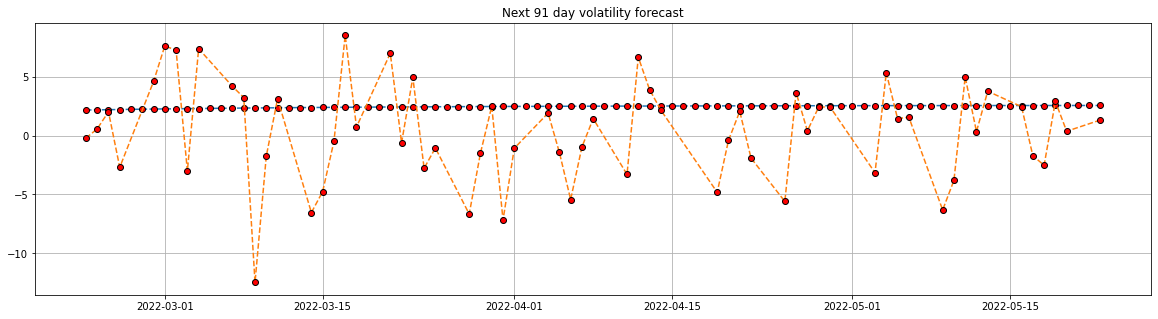
\includegraphics[width=0.6\textwidth]{Figures/Garch/crude_forecast.png}
    \caption{Brent Crude Oil Market Volatility Forecast with Realised Values}
    \label{fig:Results_table}
\end{figure}

As we can see,  there is a better fit for the trend of volatility for the GSH as opposed to the Brent Crude Oil, which is far more volatile in nature. This aligns with our initial hypothesis as the Gas Supply Hub market is more domestic in nature of trades and since most of the gas in Australia is mined and stored within Australian soil, the export is well regulated after meeting national demand. However, Brent Crude Oil is a more international market consisting of multiple European nations that rely heavily on the imports of natural gas for their industries, with a large supplier for these demands being Russia. Hence, it is expected for our GARCH forecast to underestimate the volatility of the market post-sanctions. 
\section{Cointegration Testing Between Global Oil and LNG Spot Prices}

In addition to assessing the impacts of the Russian-war in Ukraine on the volatility of both oil and LNG
prices, we assessed the long run relationship between oil and LNG prices in order to deduce whether a
shock primarily associated with one commodity (i.e., sanctions on oil production and export) may
significantly impact the price of another commodity (LNG). In order to assess this, we ran the Johansen trace
test for cointegrated relationships on weekly spot prices for Brent crude (oil) and the Henry Hub spot price
for LNG.
\medskip

Previous research into the relationship between oil and LNG has supported the existence of an “unstable”
cointegrated relationship in the United States, wherein the short-run relationship between the two
commodities is highly influenced by supply shocks such as tropical storms and seasonal factors \cite{matt1}.
This led us to examine the possible impacts a sudden demand shock (such as sanctions)
may have upon the relationship between these commodities.
\medskip

The Johansen trace test for cointegration is used to test for the existence and magnitude of cointegrating
relationships between two or more time-series. In order to run the Johansen trace test, the data sets used
must be non-stationary. As such, we ran augmented Dickey-Fuller (ADF) tests on both time series with and
without a trend. Lags were chosen using the Akaike Information Criteria (AIC) and were all equal to 1. 
\medskip

As the data in table \ref{Tab:ADF_LNG} exhibits non-stationarity without a trend, we then run the Johansen test for these time series both with a linear trend in cointegration, and without. The results are outlined in Table \ref{Tab:Johansen}.

\begin{table}[H]
\centering
% \setlength{\tabcolsep}{5pt} % Default value: 6pt
% \renewcommand{\arraystretch}{1.5} % Default value: 1
\caption{Johansen Test Results}
\begin{tabular}{c|ccc}
            & Null & Critical Value & Lag Order\\\hline\hline
No Trend & $r = 1$ & 8.34* & 2\\\hline
Linear Trend & $r = 0$ & 8.66 & 2
\end{tabular}\label{Tab:Johansen}
\\
* Significant at the 5\% level\\
** Significant at the 1\% level
\end{table}

The results from the Johansen test show that, in a model without a linear trend, there is evidence for a
cointegrating relationship between oil and LNG spot prices, however, in a model with a linear trend, there is
not. Prior research has found evidence that, at least for oil prices, there does appear to be a linear
deterministic trend \cite{matt2}. Taking this into account, we focus on the cointegrating
relationship with a linear deterministic trend, finding that there is no clear evidence of a cointegrating
relationship between these time series. For the purpose of illustration, using the coefficients retrieved from
the Johansen test with a linear trend we produce the following, clearly non-stationary plot:

\begin{figure}[H]
    \centering
    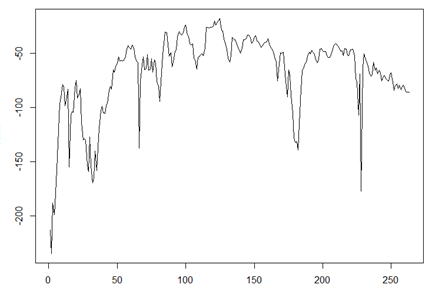
\includegraphics[width=0.6\textwidth]{Figures/Cointegration/non-stationary-plot.png}
    \caption{Non-Stationary Plot}
    \label{fig:Results_table}
\end{figure}

Running an ADF test on this model produces a test statistic that is not significant at the 5\% level ($p =
0.0972$), confirming that the relationship produced between the time series is indeed non-stationary.
Thus, we conclude that the impact of sanctions on one commodity is unlikely to significantly impact the
price of the other due to the existence of a cointegrating relationship. However it is possible that sanctions of one of
the commodities may affect the prices of the other through another channel.


\section{Conclusion}
\subsection{Summary of the Findings}
In this report, we have explored the impact of international fluctuations in gas prices on the Australian
domestic electricity market through the use of a multivariate autoregressive model of the Australian electricity
market, modelled the volatility of global oil and gas markets using a GARCH(1, 1) model in order to quantify
the impacts of the Russian war in Ukraine via a counterfactual analysis, and have examined the possibility of
a cointegrating relationship between global oil and gas spot prices.
\medskip

From these separate but related analyses, we have determined that international fluctuation in gas prices
should have a minimal impact on the National Electricity Market spot price, as there appears to be only a
moderate correlation (at best) between the aggregate gas price within the NEM and the NEM spot price,
(solar and hydro prices appears to be far more correlated with the NEM spot price). The modelling
performed on the international gas and oil markets has quantified the significant impact that the Russian
war in Ukraine has had upon the level of volatility within global oil and gas markets, with oil prices appearing
to become far more volatile as a result of (and, thus, sensitive to) the war in Ukraine. The final analysis on the
possibility of a cointegrating relationship between global oil and gas spot prices disproved the hypothesis
that there exists a cointegrating relationship between these two time series.
\subsection{Implications}
The crucial implication of these findings is that, from both an Australian and international policy perspective,
sanctions on oil appear to have a far greater impact on both domestic and international markets than
sanctions on gas (assuming these sanctions are levelled at a significant producer of both of these
commodities). They highlight the fact that oil appears to be far more sensitive to demand shocks than gas in
the Australian context, with domestic prices of oil (i.e., petrol) becoming more volatile than domestic prices
of gas (i.e., the NEM spot price).
\subsection{Future Research}
There are several future avenues of research that should be examined for a greater understanding of this
topic. Research on the impact of changes to international oil prices on the domestic Australian price of
electricity would allow for a more complete comparison of the possible impacts that sanctions on
hydrocarbons have on the Australian Electricity Market. Additionally, tests for the level of cointegration
between global oil and gas prices on their domestic Australian counterparts (the NEM spot price and
national aggregate petrol prices, respectively) may reveal underlying relationships that were not considered
in this report.

\clearpage
%---------------------- Page11: References ----------------------------
% \begin{thebibliography}{9}

 
% \end{thebibliography}
\addcontentsline{toc}{section}{References}
\bibliographystyle{plain}
\bibliography{reportbib}
\clearpage
\end{document}